%!TEX root = ../Main.tex
\subsection{Creating on-site Hamiltonian and hopping matrices for the system}
In order to calculate and visualise the band structure of the NPG within a unit cell, the on-site Hamiltonian along with its hopping matrices must be defined. The on-site Hamiltonian lies within the unit cell of the system. As the unit cell is repeated periodically the on-site Hamiltonian fills out one full period of the system. The unit cell is defined with respect given unit vectors which determine the periodicity of the system. By these definitions the elements of the hopping matrices represents hops between the repeated unit cells with respect to the periodicity. See \cref{atomrepfig} for a visual representation of the structure with its periodicity. \\
On the premise of the Tight Binding Model, the next step to find all the nearest neighbouring atoms within the given set of atom coordinates to define the on-site Hamiltonian \(\bf{h}_0\) and then define the hopping matrices \(\bf{V}\) and its conjugate \(\bf{V}^{\dagger}\). This is because the Tight Binding model only allow for hopping of electrons between nearest neighbours which in this case is the periodic boundary conditions set for the system. This can be done simply by taking what is similar to an outer product of the coordinate matrix with itself only here every combination of coordinates are subtracted not multiplied, hereafter taking the norm of all those combinations. This will produce a matrix which contain all distances between all atoms in the NPG. Once obtained a threshold will be applied to sort out the nearest neighbours within the matrix. In this specific case the coordinates given was with respect to unit vectors with a lattice constant of \(\SI{1.0}{\angstrom}\), which means that the threshold in this case should be \(\SI{1.6}{\angstrom}\) which is the inter-atomic distance for nearest neighbours in a graphene mesh. All distances above \(\SI{1.6}{\angstrom}\) will be changed to a 0-element in the on-site Hamiltonian as no hopping of electrons is possible between atoms that are more than one inter-atomic distance apart. All distances below the threshold will be changed to 1 to represent a hop between to atoms. The on-site Hamiltonian is then multiplied by at scalar which is the on-site potential \(V_{ppi}\) which in this case is \(-1\). The sorting and replacement of elements in the hamiltonian has be implemented in \cref{\npouter} as well. Now the on-site Hamiltonian is complete and the construction of the hopping matrices can begin. \\
As the on-site Hamiltonian represents a (three)two-dimensional structure one has to make sure that hopping between the nearest neighbour atoms relative to that of a repeated unit cell (on-site Hamiltonians) can described in all directions in the plane. Effectively this means that six hopping matrices should be created. One in the x-direction, one in the y-direction, one in the xy-direction and their hermitian conjugates. Graphically this corresponds to a structure of this kind:
\begin{figure}[H]
    \centering
    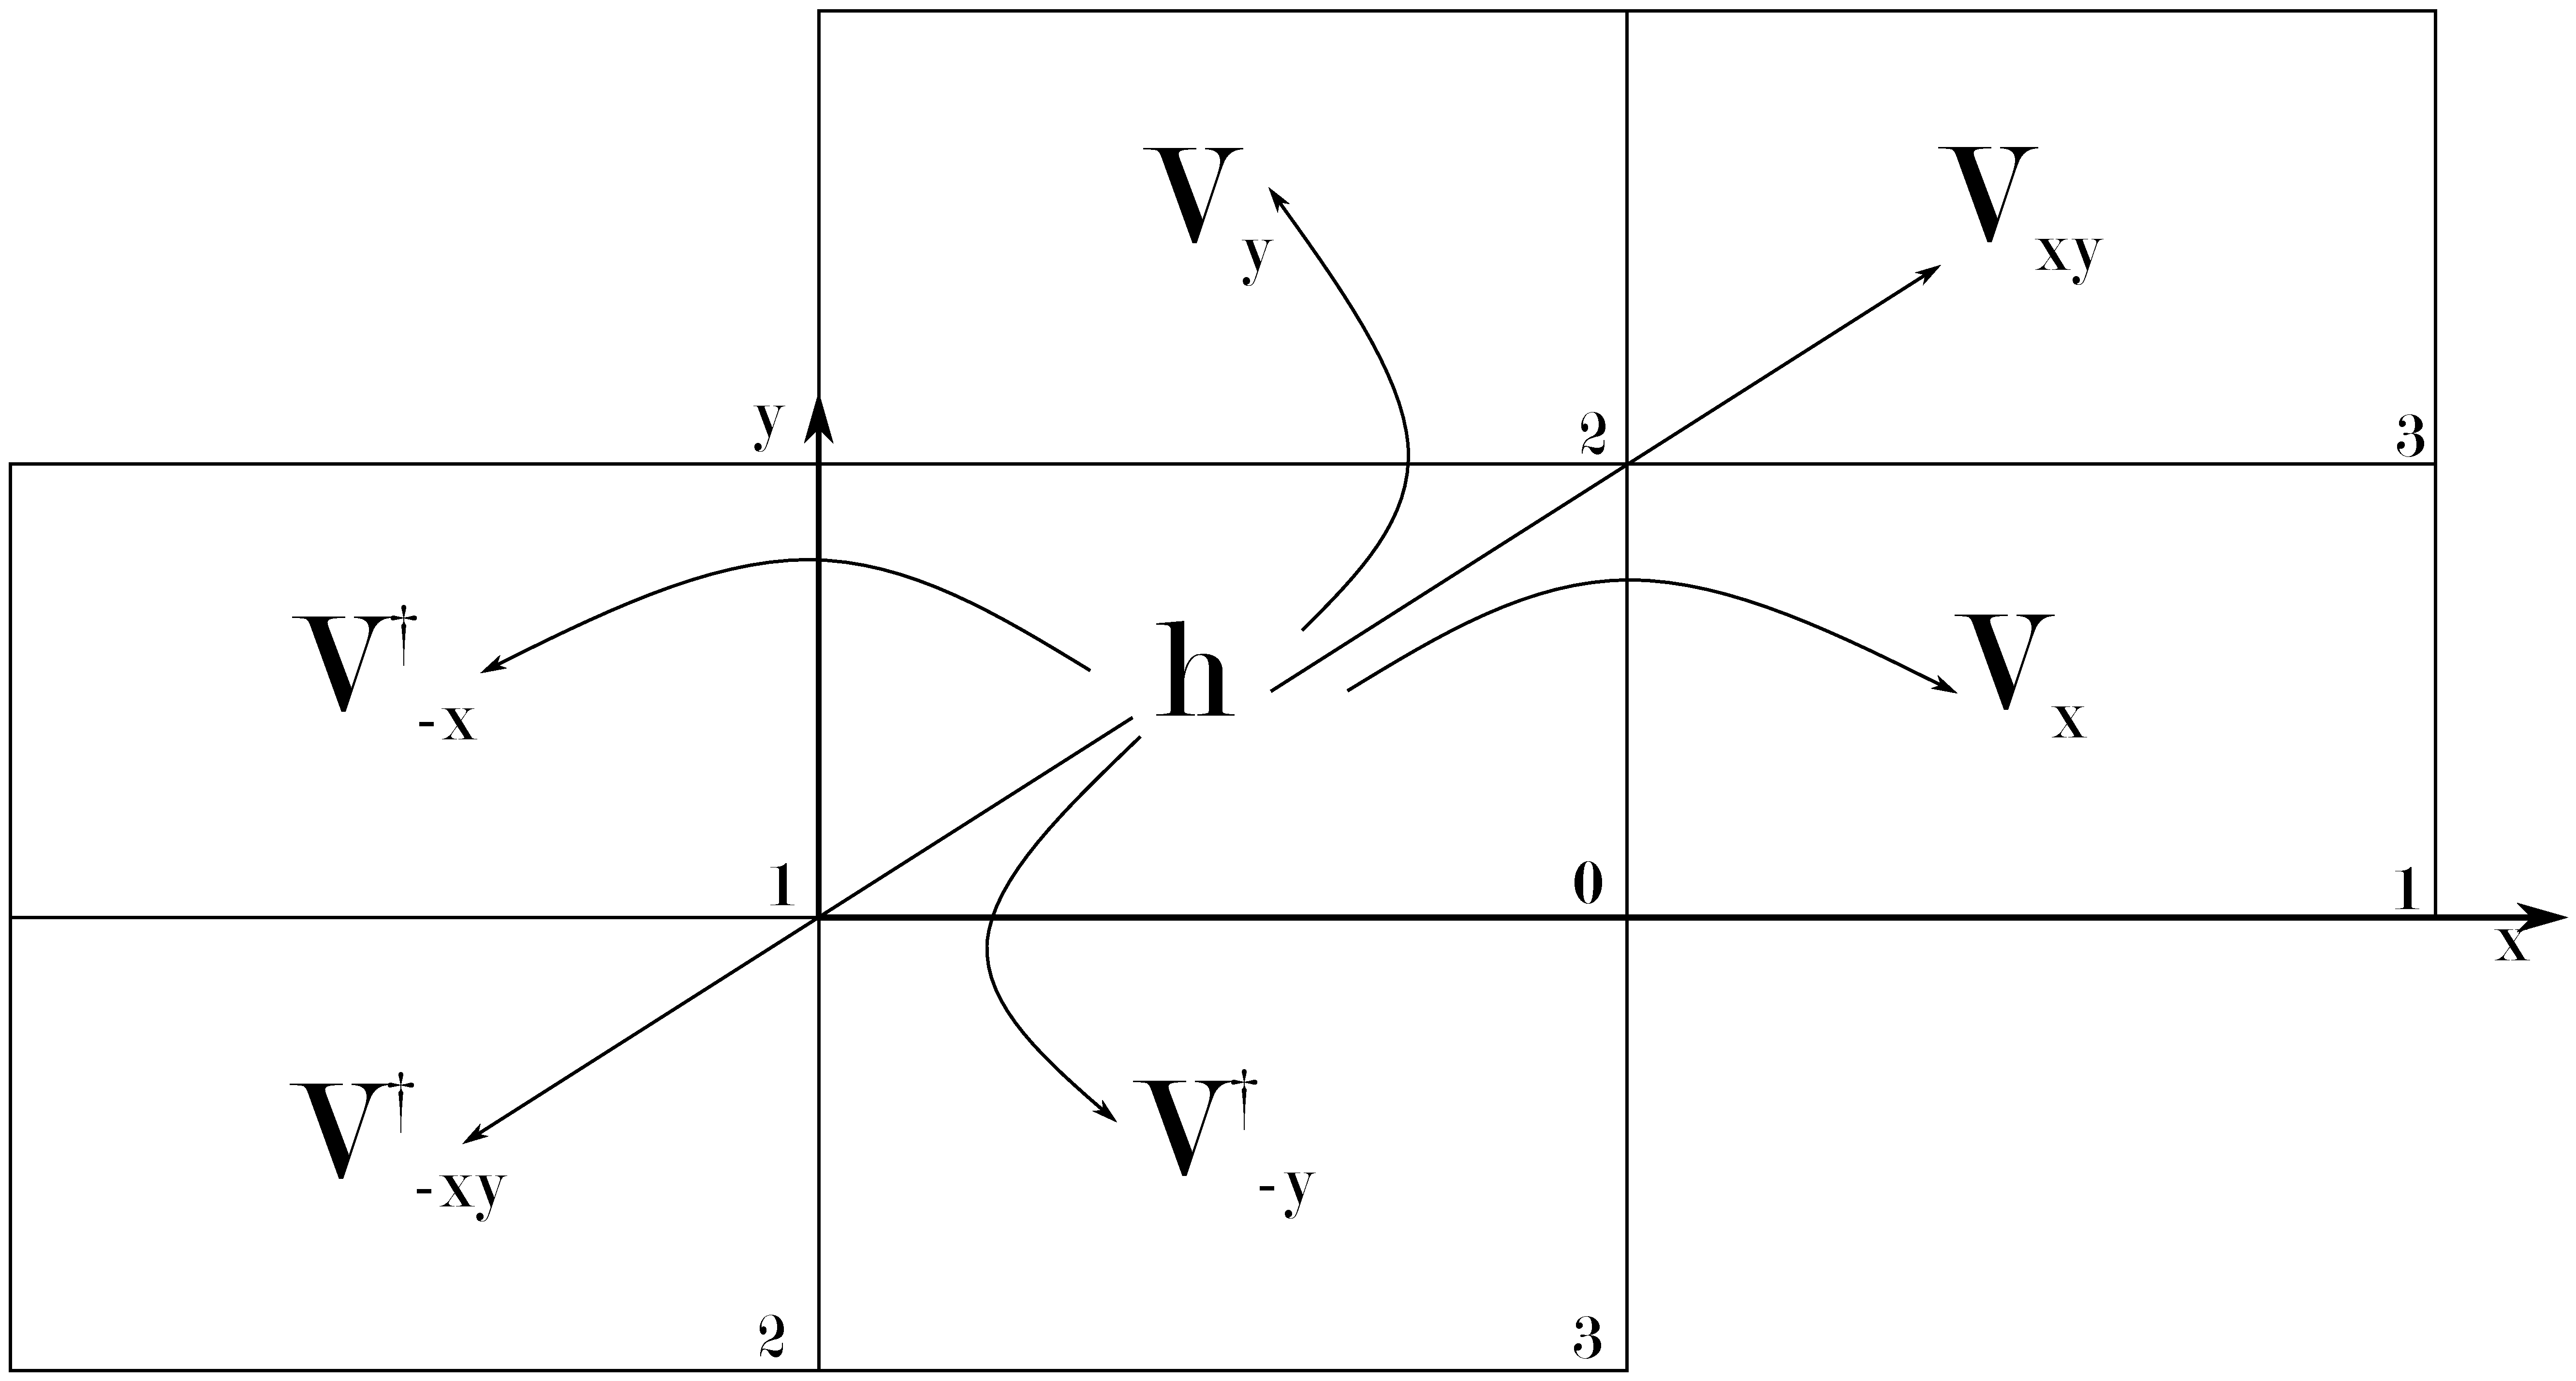
\includegraphics[width = 0.7\textwidth]{Figures/repfig.eps}
    \caption{Representative figure of how the on-site Hamiltonian along with its hopping matrices are structured}
    \label{repfig}
\end{figure}
In practice this is done by shifting the original coordinates by the given unit vectors of the system in each direction, adding the unit vector to the coordinate matrix making three new matrices. Now that three shifted matrices has been obtained, the same routine to find the distances as with the on-site Hamiltonian can be utilised, the only difference being that the outer subtraction will be between the on-site Hamiltonian and the shifted matrices respectively to make sure it is the distance between the on site Hamiltonian and the shifted matrices that is calculated. Again by replacing the distances in the shifted matrices with 1 and 0 according to the inter-atomic threshold, the hopping matrices are obtained. The three hopping matrices denoted \(\vb{V}_{1x}\), \(\vb{V}_{2y}\) and \(\vb{V}_{3xy}\) represent hopping in the "forward" direction (left-to-right). To create the hopping matrices hopping in the "backwards" (right-to-left) direction one simply has to transpose the hopping matrices. These matrices are denoted with a dagger: \(\vb{V}_{1x}^{\dagger}\), \(\vb{V}_{2y}^{\dagger}\) and \(\vb{V}_{3xy}^{\dagger}\). \cref{matrixmap} is a figure of the resulting matrix-maps from the calculation, stitched together like in \cref{repfig}.

\begin{figure}[H]
    \centering
    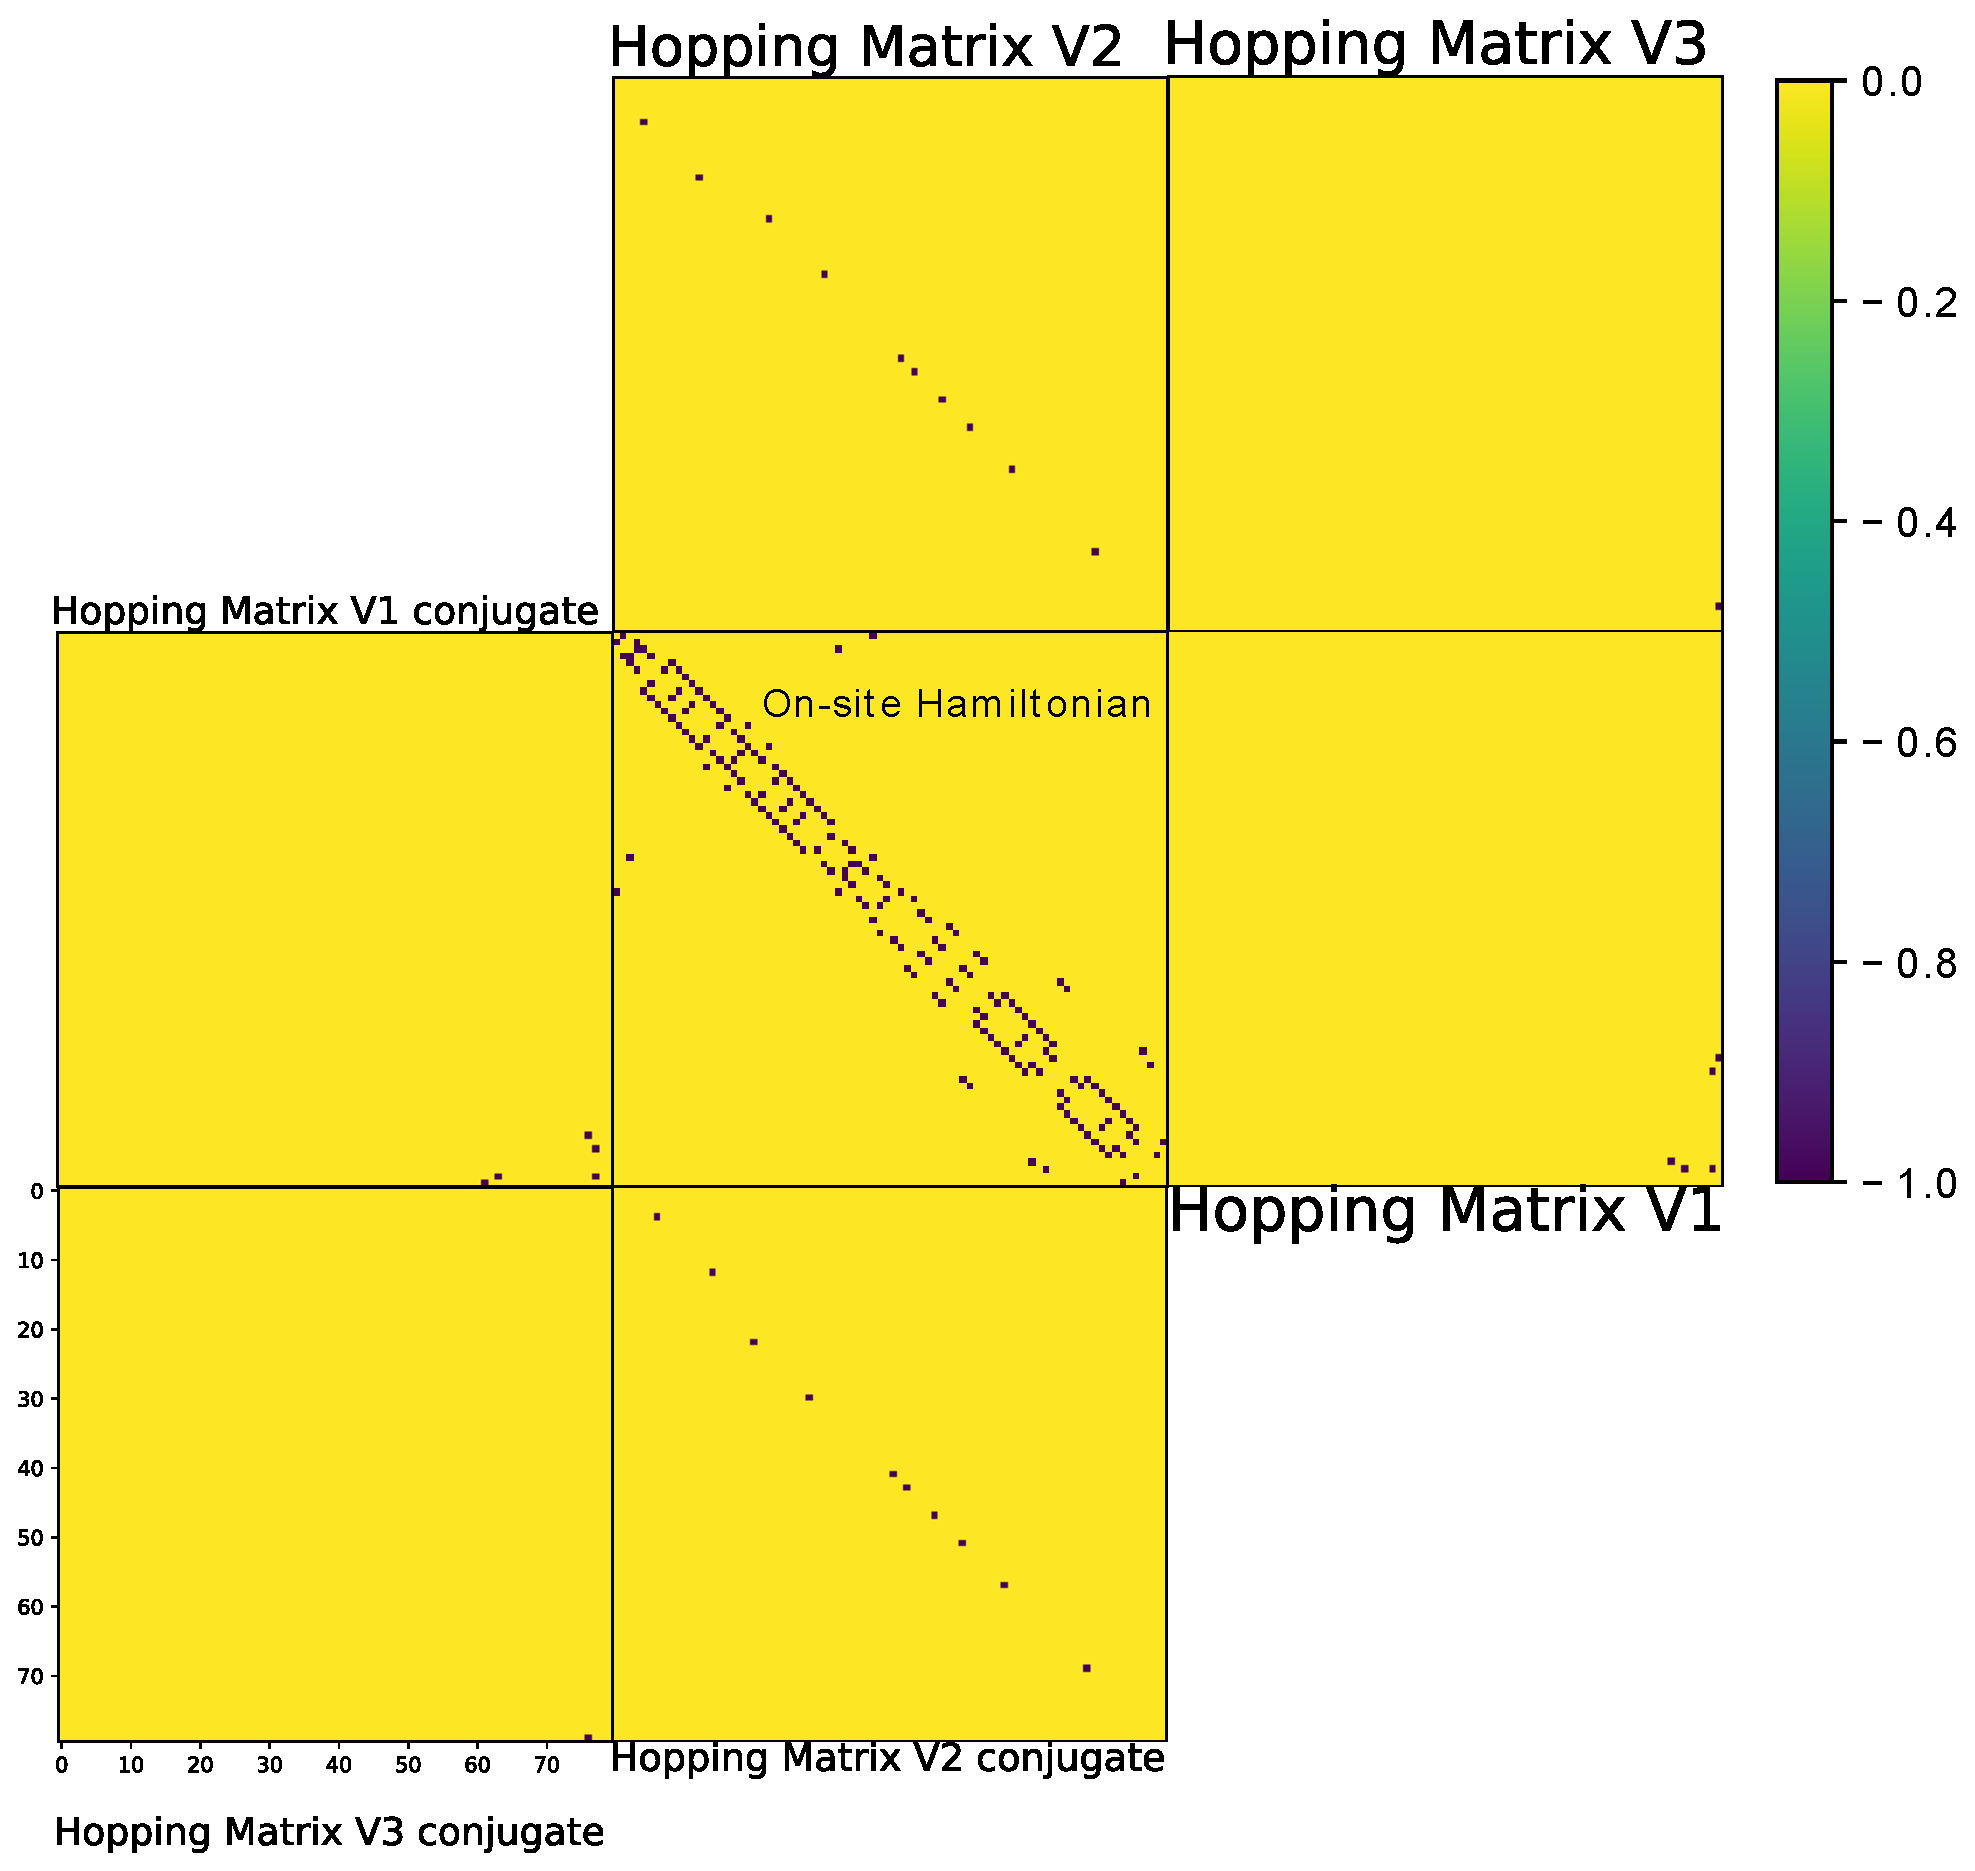
\includegraphics[width=\textwidth]{Figures/Matrixmap.eps}
    \caption{Matrix maps from calculation on the NPG. The on-site Hamiltonian along with all its hopping matrices are stitched together like the representative figure \cref{repfig}. All the dark spots represents a hopping of an electron to its nearest neighbour.}
    \label{matrixmap}
\end{figure}
\begin{figure}[H]
    \centering
    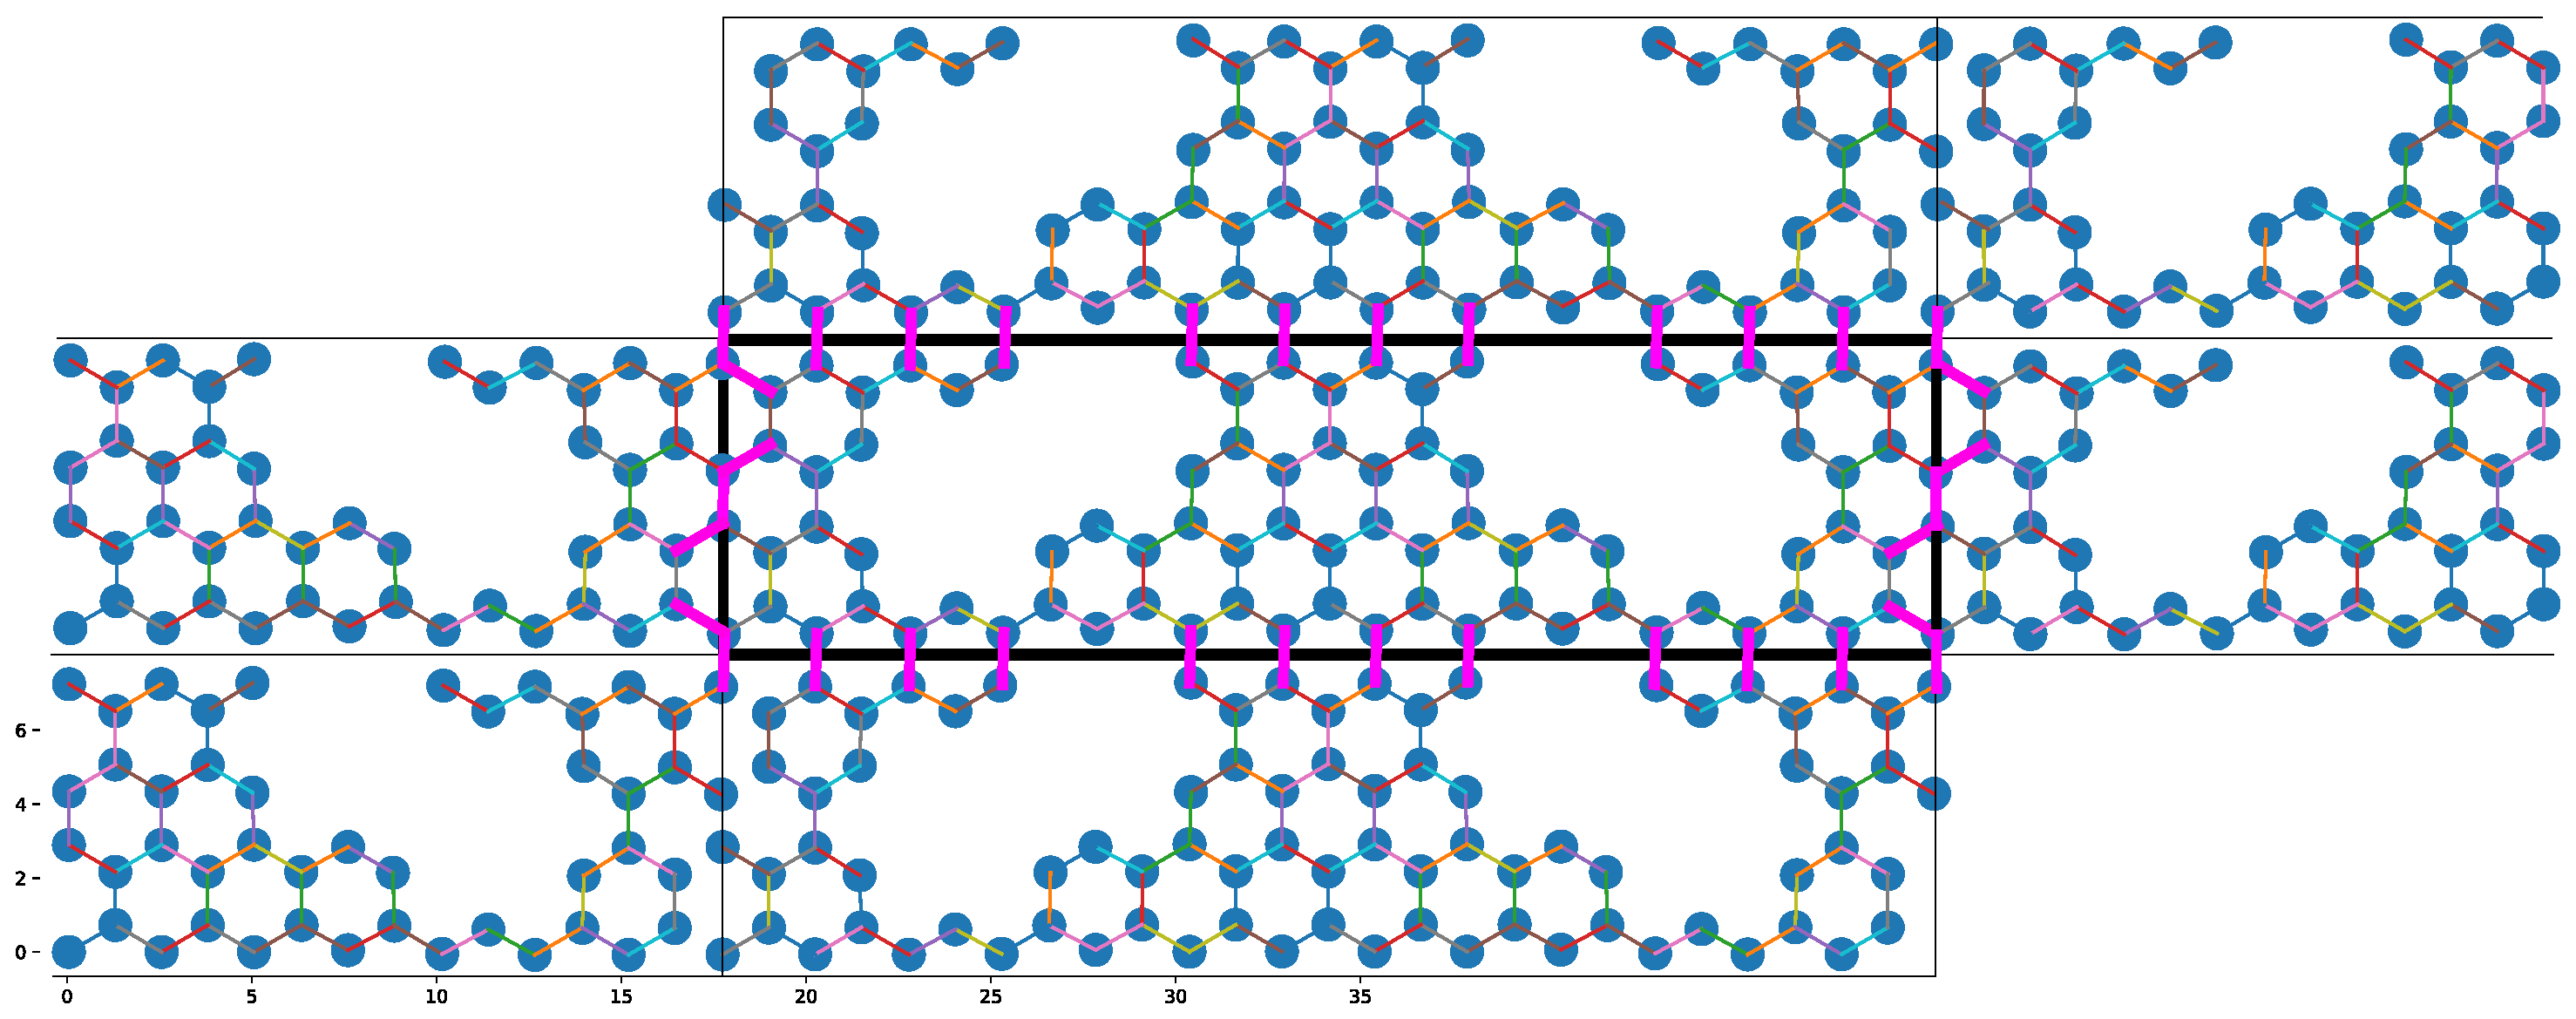
\includegraphics[width=\textwidth]{Figures/representativestructure2.eps}
    \caption{Visual representation of the periodic NPG-structure. The atoms surrounded by the black box in the centre represents the unit cell. The neighbouring boxes are unit cells repeated periodically. Note that the two cells left and right with respect to the centre cell has been cut in half for figure space. The pink lines crossing the black box represents the link between the nearest neighbours in the adjacent cell. Note how this representation corresponds to that of \cref{matrixmap}. There is more 'hopping' when going up and down, than left or right and the two cells at the diagonal only have one atom which is nearest neighbour to the centre cell which corresponds to the one hopping elements in \cref{matrixmap}.}
    \label{atomrepfig}
\end{figure}
\subsection{Defining the full Hamiltonian and solving the Schrodinger equation}\label{FullHam}
Now that the on-site Hamiltonian along with its hopping matrices has been defined, the next step is to create the full Hamiltonian in order to solve the Schrodinger equation for system, which is a eigen-value/vector problem. In essence the full Hamiltonian denoted \(\vb{H}\) is a sum of the on-site Hamiltonian and its corresponding hopping matrices multiplied by a complex exponential function that has the appropriate phase relative to the hopping matrix:
\begin{align}\label{hamileq}
\vb{H}(k_x,k_y) = \vb{h}_0 &+ (\vb{V}_{1x}e^{-ik_x} + \vb{V}_{1x}^{\dagger}e^{ik_x}\\ \nonumber
& + \vb{V}_{2y}e^{-ik_y} + \vb{V}_{2y}^{\dagger}e^{-ik_y}\\ 
& + \vb{V}_{3xy}e^{-ik_x}e^{-ik_y} + \vb{V}_{3xy}^{\dagger}e^{ik_x}e^{ik_y}) \nonumber
\end{align}
Here \(k\) represents a continuous variable between 0 and \(\pi\) along the x- and y-axis in inverse space.
Using the full Hamiltonian, the Schrodinger equation can be solved
\begin{align}
    \vb{H}(k_x,k_y)\vb*{\phi}_{k} = \vb*{\epsilon}_n (k_x,k_y) \vb*{\phi}_k
\end{align}
In practice this is all done by defining a function that takes the on-site Hamiltonian, the hopping matrices, and \(k\) (\(x,y\)) as inputs and outputs the eigenvalues, using numpy's \textit{numpy.linalg.eigh}. The number of eigenvalues in the output corresponds to the dimension of the full Hamiltonian. In \cref{fullhamil} the code for the function is shown.\begin{listing}[ht]
    \centering
    \im{Listings/Functions.py}{52}{61}
    \caption{Function producing the full hamiltonian, corresponding to \cref{hamileq}}
    \label{fullhamil}
\end{listing}As the eigenvalues corresponds to the eigenenergies of the system, the band structures can be plotted.
\subsection{Plotting the band structures}
The continuous variable \(k\) extends in two directions (\(-k_{x}\)) and (\(k_{y}\)) which corresponds to lengths between the symmetry points \(X\), \(\Gamma\) and \(Z\) in the Brillouin zone, with \(\Gamma\) being the zero-point. It is therefore necessary to make two plots, one for each pair of symmetry points. The y-values in each plot corresponds to the eigenvalues obtained by the function described in \cref{FullHam}. Each x-value between \(\Gamma\), \(X\) and \(\Gamma\), \(Z\) therefore has associated with it the amount of y-values which the dimension of full Hamiltonian dictates. F.ex. if the full Hamiltonian has dimension \(80\times80\) there is 80 eigenvalues associated with it and the amount of y-values for each x-value between \(\Gamma\), \(X\) and \(\Gamma\), \(Z\) is 80. In this specific case, the full Hamiltonian for obtaining the eigenvalues that corresponds to \(X\) and \(Z\) are:
\begin{align}\label{hamilxgamma}
X: \ \vb{H}_{X} = \vb{h}_0 + (\vb{V}_{1x}e^{ik_x} + \vb{V}_{1x}^{\dagger}e^{-ik_x} + \vb{V}_{2x} + \vb{V}_{2x}^{\dagger} + \vb{V}_{3xy}e^{ik_x} + \vb{V}_{3xy}^{\dagger}e^{-ik_x})\\
Z: \ \vb{H}_{Z} = \vb{h}_0 + (\vb{V}_{1x} + \vb{V}_{1x}^{\dagger} + \vb{V}_{2x}e^{-ik_y} + \vb{V}_{2x}^{\dagger}e^{ik_y} + \vb{V}_{3xy}e^{-ik_y} + \vb{V}_{3xy}^{\dagger}e^{ik_y})
\end{align}
Using the eigenvalues as y-values in the two plots, putting the two plots together  will yield a full plot of the band structure shown in \cref{Fab}.
\begin{figure}[H]
    \centering
    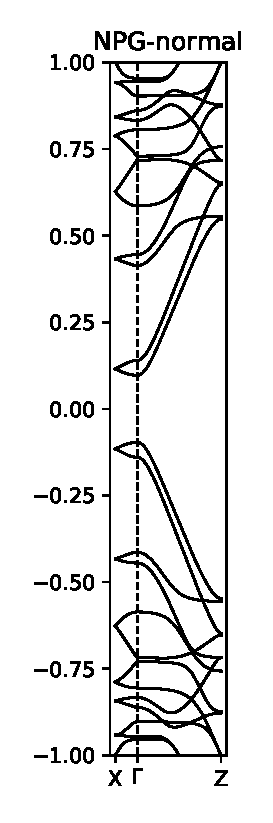
\includegraphics{Figures/FabNPGBS.eps}
    \caption{Plot showing the band structure in the energy range -1 to 1 for NPG with normal bridges between symmetry points \(X\) and \(Z\) with respect to \(\Gamma\)}
    \label{Fab}
\end{figure}

\begin{figure}
    \centering
    \begin{subfigure}[b]{0.3\textwidth}
        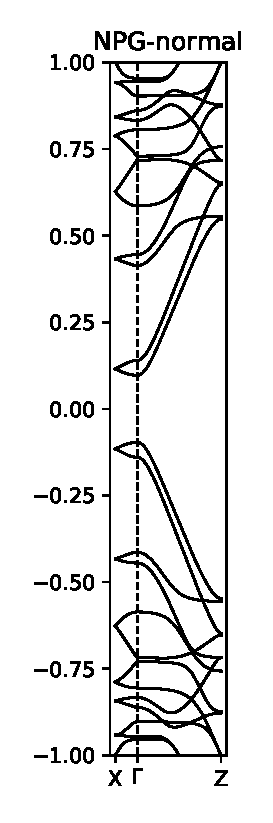
\includegraphics[width=\textwidth]{Figures/FabNPGBS.eps}
                \caption{Plot showing the band structure in the energy range -1 to 1 for NPG with normal bridges between symmetry points \(X\) and \(Z\) with respect to \(\Gamma\)}
        \label{Fabbs}
    \end{subfigure}
    ~ %add desired spacing between images, e. g. ~, \quad, \qquad, \hfill etc.
      %(or a blank line to force the subfigure onto a new line)
    \begin{subfigure}[b]{0.3\textwidth}
        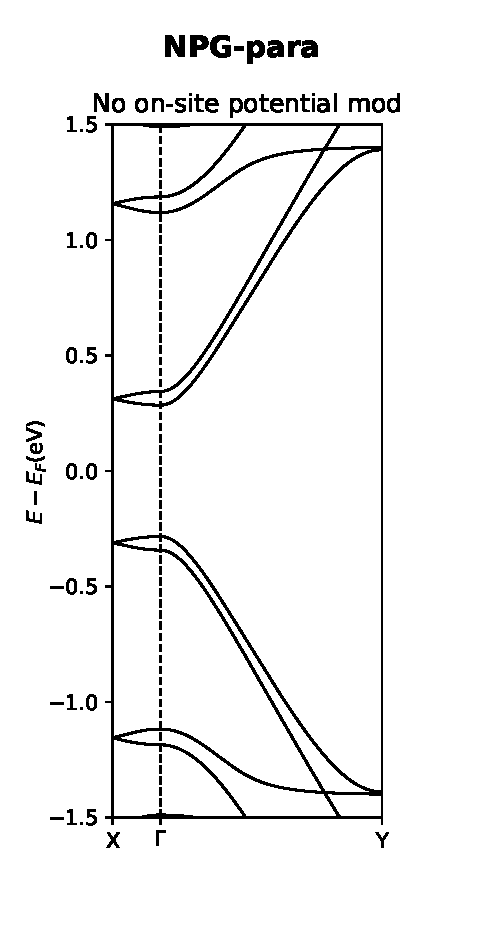
\includegraphics[width=\textwidth]{Figures/paraNPGBS.eps}
        \caption{Plot showing the band structure in the energy range -1 to 1 for NPG with para bridges between symmetry points \(X\) and \(Z\) with respect to \(\Gamma\)}
        \label{parabs}
    \end{subfigure}
    ~ %add desired spacing between images, e. g. ~, \quad, \qquad, \hfill etc.
    %(or a blank line to force the subfigure onto a new line)
    \begin{subfigure}[b]{0.3\textwidth}
        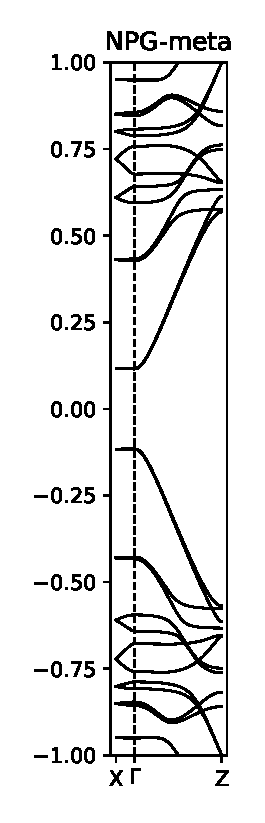
\includegraphics[width=\textwidth]{Figures/metaNPGBS.eps}
        \caption{Plot showing the band structure in the energy range -1 to 1 for NPG with meta bridges between symmetry points \(X\) and \(Z\) with respect to \(\Gamma\)}
        \label{metabs}
    \end{subfigure}
    \caption{Figure showing para, meta and normal NPG band structures}\label{allbands}
\end{figure}
